\section{Auswertung}
\label{sec:Auswertung}
\subsection{Bestimmung des lokalen Erdmagnetfeldes}
Für die Bestimmung des Erdmagnetfeldes werden die Magnetfeldstärken des
Sweep- und Horizontalfeldes in Abhängigkeit der Resonanzfrequenz gemessen.
Die gemessenen Messwerte werden in der Tabelle \ref{tabmess1} dargestellt.
 \begin{table}
   \centering
   \caption{Position der Resonanzstellen für verschiedene Frequenzen}
   \label{tabmess1}
   \sisetup{parse-numbers=false}
   \begin{tabular}{c|c|c|c|c}
     \toprule
    $f$ in Hz & Sweep 1& Horizontal 1 & Sweep 2&Horizontal 2 \\
     \midrule
     100 &  5.66 &  6.84  & 0   &   0   \\
     200 &  5.78 & 7.13  & 0.15 &  0.15  \\
     300 &  5.43 & 8.96  & 0.20 &  0.20 \\
     400 &  4.24 & 9.01  & 0.28 &  0.28 \\
     500 &  2.41 & 8.32  & 0.38 &  0.38 \\
     600 &  1.67 & 8.71  & 0.44 &  0.44 \\
     700 &  0.98 & 9.28  & 0.52 &  0.52 \\
     800 &  3.34 & 7.73  & 0.52 &  0.64 \\
     900 &  2.26 & 4.76  & 0.60 &  0.78 \\
     1000 & 4.10 & 6.01  & 0.61 &  0.83 \\
     \bottomrule
   \end{tabular}
 \end{table}
Die in der Tabelle dargestellten Positionen der Resonantstellen geben an, wie
viel Strom durch die Spulen fließt. Zur Berechnung der Stromstärke müssen
die Positionen der Sweepfelder und der Horizontalfelder mit den Faktoren
$0.1$ und $0.3$ multipliziert werden. Mit Hilfe dieser berechneten Stromstärken
und der Helmholzgleichung \eqref{holziholziholz} können die Magnetfeldstärken der Sweep- und
Horizontalfeldstärken berechnet werden.
\begin{align}
\label{holziholziholz}
B=\frac{I\cdot 8\mu_0}{R\sqrt{125}}
\end{align}
Anschließend werden die Magnetfeldstärken der Sweep- und Horizontalspule addiert
und gegen die Frequenz $f$ aufgetragen. An diese Werte kann eine
Funktionsanpassungen durchgeführt werden, dieser Plot wird in Abbildung
\ref{plot1} dargestellt.

\begin{figure}
\centering
\includegraphics{ressources/fit_reso.pdf}
\caption{Messwerte und Darstellung der Fitgergebnisse zur Berechnung
der Land$\grave{\text{e}}$-Faktoren und des Erdmagnetfeldes}
\label{plot1}
\end{figure}

Die Steigung der linearen Funktion lässt sich mit Hilfe der Gleichung \eqref{eq:hnu}
berechnen, es folgt:
\begin{align}
    \label{Lande}
    m=\frac{h}{g_\text{F}\mu_\text{B}}
\end{align}
Die Werte des linearen Fitmodells liegen bei:
\begin{align}
    \nonumber
    m_1&=1.54\cdot 10^{-10} \pm 8\cdot 10^{-12}\\
    \nonumber
    m_2&=2.26\cdot 10^{-10} \pm 7\cdot 10^{-12}\\
    \nonumber
    b_1&=3.4\cdot 10^{-5} \pm 5\cdot 10^{-6}\\
    \nonumber
    b_2&=3.3\cdot 10^{-5} \pm 4\cdot 10^{-6}
\end{align}
Die Y-Achsenabschnitte der Fits entsprechen der horizontalen Komponenten
des Erdmagnetfeldes kann als Horizontalkomponente des Erdmagnetfeldes
identifiziert werden:
\begin{align}
    \nonumber
    B_{\text{hor.}1}&=(34 \pm 5)\, \mu\text{T}\\
    \nonumber
    B_{\text{hor.}2}&=(33 \pm 4)\, \mu\text{T}
\end{align}
Die vertikale Komponente des Erdmagnetfeld wird mit einer seperaten Spule
ausgeglichen, der durchflossene Strom lag bei $I=0.15\,\text{A}$. Die
Berechnung der Magnetfeldstärke der vertikalen Komponente erfolgt mit der Gleichung
\eqref{holziholziholz}:

\begin{align}
    B_\text{vert.}=(23 \pm 2)\, \mu \text{T}
\end{align}
Für das gesamte Magnetfeld der Erde folgt:
$$B_\text{Erde}=(41\pm 5 )\, \mu \text{T}.$$

Die Bestimmung der Land$\grave{\text{e}}$-Faktoren der beiden Isotope
erfolgt aus der Steigung der
linearen Fits, dazu wird die Gleichung \eqref{Lande} nach $g_\text{F}$
umgestellt, daraus konnten folgende Faktoren ermittelt werden:
\begin{align}
    g_{\text{F}1}=0.46 \pm 0.02 \\
    g_{\text{F}2}=0.32 \pm 0.01
\end{align}

% Sämtliche im Folgenden durchgeführten Ausgleichsrechnungen werden mit der \emph{curve fit} Funktion aus dem für \emph{Python} geschriebenen package \emph{NumPy}\cite{scipy} durchgeführt. Fehlerrechnungen werden mit dem für \emph{Python} geschriebenen package \emph{Uncertainties}\cite{uncertainties} ausgeführt.

% % Examples
% \begin{equation}
%   U(t) = a \sin(b t + c) + d
% \end{equation}
%
% \begin{align}
%   a &= \input{build/a.tex} \\
%   b &= \input{build/b.tex} \\
%   c &= \input{build/c.tex} \\
%   d &= \input{build/d.tex} .
% \end{align}
% Die Messdaten und das Ergebnis des Fits sind in Abbildung~\ref{fig:plot} geplottet.
%
% %Tabelle mit Messdaten
% \begin{table}
%   \centering
%   \caption{Messdaten.}
%   \label{tab:data}
%   \sisetup{parse-numbers=false}
%   \begin{tabular}{
% % format 1.3 bedeutet eine Stelle vorm Komma, 3 danach
%     S[table-format=1.3]
%     S[table-format=-1.2]
%     @{${}\pm{}$}
%     S[table-format=1.2]
%     @{\hspace*{3em}\hspace*{\tabcolsep}}
%     S[table-format=1.3]
%     S[table-format=-1.2]
%     @{${}\pm{}$}
%     S[table-format=1.2]
%   }
%     \toprule
%     {$t \:/\: \si{\milli\second}$} & \multicolumn{2}{c}{$U \:/\: \si{\kilo\volt}$\hspace*{3em}} &
%     {$t \:/\: \si{\milli\second}$} & \multicolumn{2}{c}{$U \:/\: \si{\kilo\volt}$} \\
%     \midrule
%     \input{build/table.tex}
%     \bottomrule
%   \end{tabular}
% \end{table}
%
% % Standard Plot
% \begin{figure}
%   \centering
%   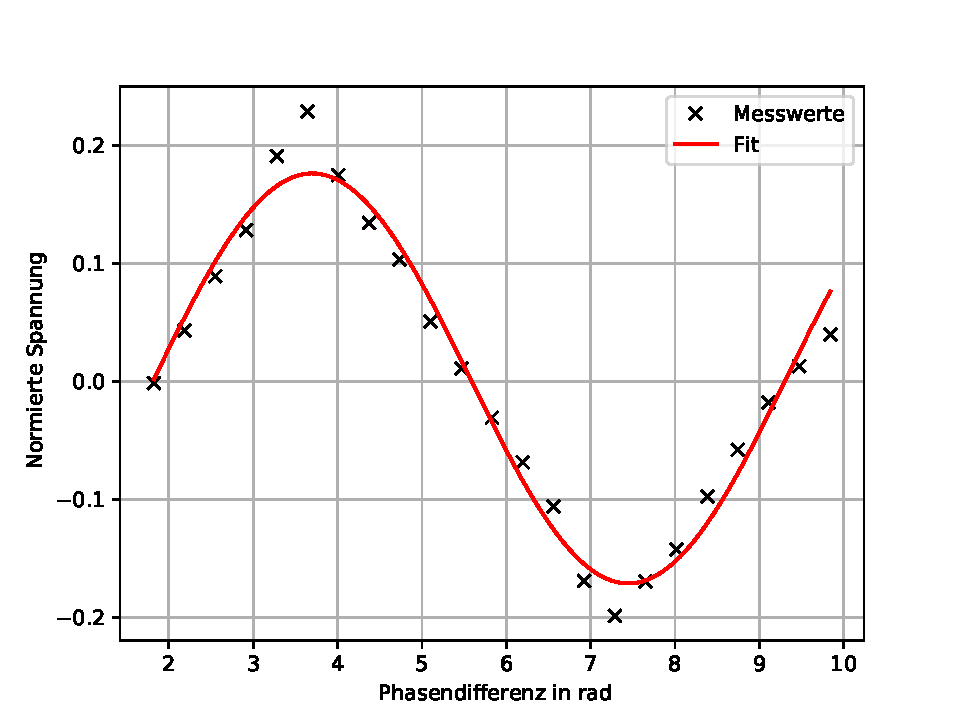
\includegraphics{build/plot.pdf}
%   \caption{Messdaten und Fitergebnis.}
%   \label{fig:plot}
% \end{figure}
%
% 2x2 Plot
% \begin{figure*}
%     \centering
%     \begin{subfigure}[b]{0.475\textwidth}
%         \centering
%         \includegraphics[width=\textwidth]{Abbildungen/Schaltung1.pdf}
%         \caption[]%
%         {{\small Schaltung 1.}}
%         \label{fig:Schaltung1}
%     \end{subfigure}
%     \hfill
%     \begin{subfigure}[b]{0.475\textwidth}
%         \centering
%         \includegraphics[width=\textwidth]{Abbildungen/Schaltung2.pdf}
%         \caption[]%
%         {{\small Schaltung 2.}}
%         \label{fig:Schaltung2}
%     \end{subfigure}
%     \vskip\baselineskip
%     \begin{subfigure}[b]{0.475\textwidth}
%         \centering
%         \includegraphics[width=\textwidth]{Abbildungen/Schaltung4.pdf}    % Zahlen vertauscht ... -.-
%         \caption[]%
%         {{\small Schaltung 3.}}
%         \label{fig:Schaltung3}
%     \end{subfigure}
%     \quad
%     \begin{subfigure}[b]{0.475\textwidth}
%         \centering
%         \includegraphics[width=\textwidth]{Abbildungen/Schaltung3.pdf}
%         \caption[]%
%         {{\small Schaltung 4.}}
%         \label{fig:Schaltung4}
%     \end{subfigure}
%     \caption[]
%     {Ersatzschaltbilder der verschiedenen Teilaufgaben.}
%     \label{fig:Schaltungen}
% \end{figure*}
